\documentclass{article}
\usepackage{arxiv}
\usepackage[utf8]{inputenc}
\usepackage[T1]{fontenc}
\usepackage{hyperref}
\usepackage{url}
\usepackage{booktabs}
\usepackage{amsmath}
\usepackage{graphicx}
\usepackage{microtype}
\title{MIMESIS: Geographic stability in Earth--Moon--Mars terrain analogue screening}
\author{Arjun Vijay Prakash\\
Grade XI, City Montessori School, Kanpur Road\\
Lucknow, India\\
\url{https://arjuncodess.is-a.dev/}}
\date{November 15, 2026}
\renewcommand{\shorttitle}{MIMESIS: geographic stability}
\renewcommand{\headeright}{Research draft}
\renewcommand{\undertitle}{Exploratory research report}
\hypersetup{pdftitle={MIMESIS: Geographic stability in terrain analogue screening},pdfauthor={Arjun Vijay Prakash},colorlinks=true,linkcolor=black,urlcolor=blue,citecolor=black}
\begin{document}
\maketitle
\begin{abstract}
Terrain rankings can change without identifying a different physical landscape. We compare two scoring contracts at 500 m and 1,000 m support for six Moon and Mars targets using 3,693 overlapping NASADEM windows in the Namib and Atacama. The first contract uses four scaled terrain descriptors; the second combines four descriptor groups with a maximum over 35 sensitivity scenarios. Within a contract, the largest displacement of a winning center is 24.19 km. Between contracts, winners for Jezero and Syrtis move between Namibia and Chile, by 8,349--8,484 km. For Nili Fossae, the scalar top tens share no candidate identifiers, yet their winners are only 3.00 km apart and their 20 km footprints have intersection-over-union 0.739. Five of ten top-ten pairs can be matched one-to-one within 10 km. We release geographic shortlists selected by minimizing the worse rank across supports, with source hashes and reproducible calculations. This post hoc regional result separates identifier turnover, geographic turnover and scoring assumptions. It does not establish a new geological analogue or a safe base location. Independent source-quality and geological checks remain necessary, as illustrated by the accompanying MOLA sampling and lunar pit experiments.
\end{abstract}
\keywords{terrestrial analogues \and NASADEM \and MOLA \and LOLA \and geographic stability}

\section{Research question and contribution}
An Earth location can support a specific exploration task without reproducing an entire lunar or Martian environment. Analogue-site frameworks emphasize selecting for a science or engineering objective rather than an overall impression of fidelity \cite{framework}. MIMESIS addresses regional terrain mapping: comparing relief, slope distributions, terrain organization and surrounding context. It does not estimate rover traction, construction safety or resource abundance.

Adjacent overlapping windows can exchange ranks while retaining much of the same ground. Conversely, two scoring contracts can choose different continents even when each appears stable under a change of support. We test both possibilities using existing Earth--Moon--Mars measurements. The contribution is an original geographic follow-up within this project, with candidate coordinates and explicit limits. We do not claim priority for sensitivity analysis, geographic matching or minimax selection as general methods.

All six targets and both Earth regions were inspected during earlier development. Labels originally called held out no longer confer independent validation. This follow-up is exploratory. Earlier global eligibility, point-support, spectral and feature-scale records use different pools and cannot be combined into a larger apparent sample.

\section{Data and methods}
\subsection{NASA observations and spatial support}
Earth descriptors originate in NASADEM; Mars descriptors use MGS MOLA gridded topography, and lunar descriptors use LRO LOLA \cite{nasadem,mola,lola}. The frozen bundle contains 1,844 Atacama and 1,849 Namib windows. Each local square is 20 km wide, its contextual square is 80 km wide, and candidate centers are separated by 3 km. We compare 500 m and 1,000 m analysis support. Analysis spacing does not imply native source resolution or common information content.

The references are Jezero crater, Nili Fossae, Isidis Planitia and Syrtis Major on Mars, and Taurus--Littrow and the Shackleton rim on the Moon. Descriptors represent fixed study windows, not entire geological provinces. Absolute elevation is excluded from cross-body discrepancy. Both supports must have complete feature vectors. Original products, body-specific coordinates, quality masks and ancestry remain in the source manifests.

\subsection{Two scoring contracts}
The scalar contract uses relief, median slope, upper-decile slope and residual roughness. Relief and roughness use $\log_{10}(x+1)$; slopes remain in degrees. Equal-weight root-mean-square discrepancy uses fixed interquartile scales from the 500 m Earth pool, with standard deviation as fallback. This independently implemented four-variable adaptation retains the provenance of its baseline \cite{terrainfinder}; it differs from that six-variable implementation.

The multigroup contract combines slope-histogram Wasserstein distance, relief and terrain position, roughness and organization, and multiscale context. Weights are 0.40, 0.25, 0.15 and 0.20. Scalar losses use $\min(1,|x-y|/\tau)^2$ with declared engineering tolerances. The score is the maximum over 35 scenarios, including weight perturbations, alternate support and mask erosion. Neither contract has independent geological relevance calibration.

The contracts differ in observables, normalization, weighting and aggregation. This comparison cannot attribute a change to one ingredient. Alternate support already enters the multigroup score; small support shifts there are partly a design consequence, not independent proof of superiority.

\subsection{Geographic comparison and shortlist rule}
Candidates are sorted by score, with ID as the stable tie-breaker. We measure exact top-ten identifier overlap, WGS84 geodesic displacement of winning centers, and square footprint intersection-over-union, $A_{\cap}/A_{\cup}$, in the shared regional azimuthal-equidistant measurement projection. Namibia and Chile are disjoint pools.

Top-ten geographic comparison uses maximum-cardinality one-to-one matching at 5, 10, 20 and 40 km center-distance radii, with total distance breaking ties. A nearby candidate cannot count twice. These radii are exploratory diagnostics relative to the window size, not field-operation tolerances.

For each target and contract, a shortlist entry minimizes the worse full-pool rank across supports. Rank sum and ID break ties, in that order:
\begin{equation}
c^*=\arg\min_c\left(\max\{r_{500}(c),r_{1000}(c)\},\ r_{500}(c)+r_{1000}(c),\ \operatorname{ID}(c)\right).
\end{equation}
This rule avoids choosing a support after seeing its winner. It produces a terrain-screening location, not source qualification or geological validation.

\section{Results}
\subsection{Identifier turnover and shared physical ground}
The scalar contract changes its first-ranked window for four of six targets. Exact top-ten overlaps are 6, 0, 9, 7, 6 and 6 in Figure~\ref{fig:geography}'s order. Winning-center displacements are 24.19, 3.00, 0, 3.00, 0 and 3.00 km. All six scalar winners remain in their respective Earth region when support changes.

For Nili Fossae, no top-ten ID survives, but the winners' footprint intersection-over-union is 73.91\%. Five top-ten pairs match one-to-one within 10 km; seven match within 40 km. Exact turnover therefore exaggerates geographic replacement in this case. It does not establish complete stability: half the top ten cannot be paired within 10 km. The minimax-rank candidate has ranks 17 and 19, outside both top tens.

\begin{figure}[htbp]
\centering
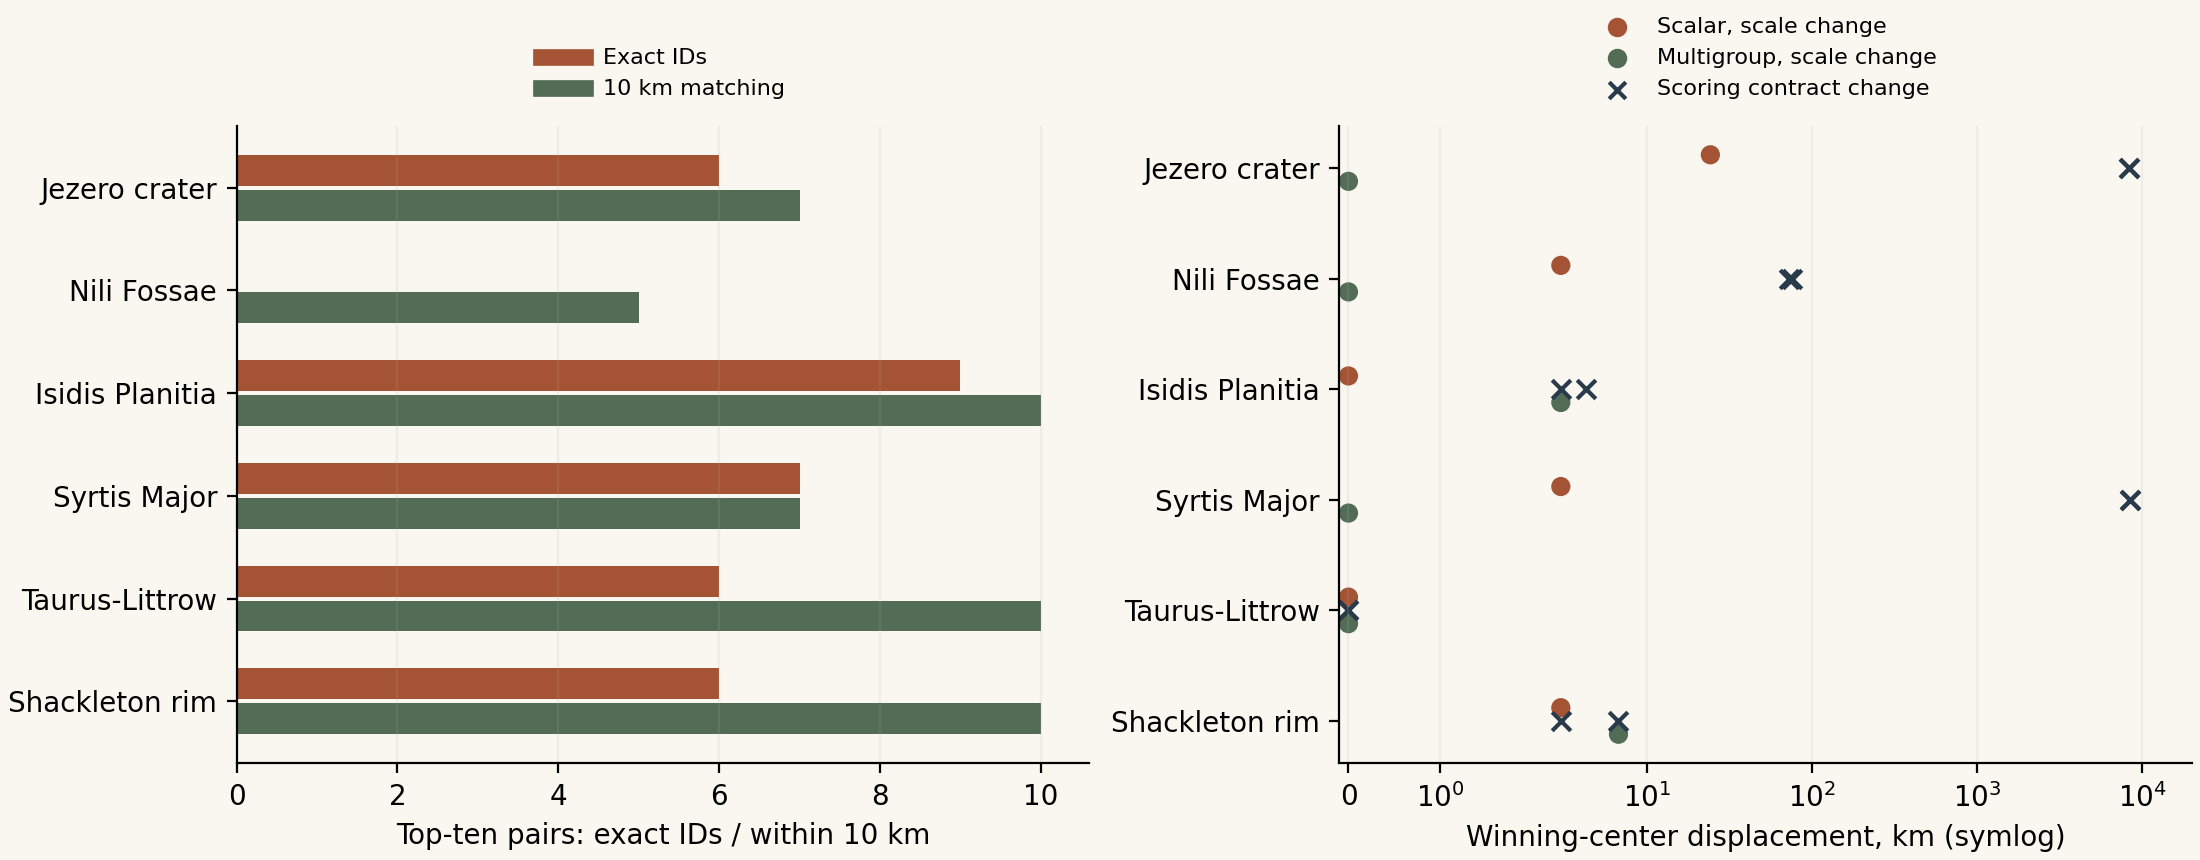
\includegraphics[width=\linewidth]{site-stability.png}
\caption{Left: exact top-ten overlap and maximum one-to-one matches within 10 km for the scalar contract. Right: winning-center displacement under support changes within each contract and contract changes at fixed support. Distance uses a symmetric-logarithmic axis, linear near zero. Conditions are correlated diagnostics, not independent replicates.}
\label{fig:geography}
\end{figure}

\subsection{Scoring assumptions can change the selected continent}
Across twelve within-contract support comparisons, maximum displacement is 24.19 km and median displacement is 1.50 km. Across twelve between-contract comparisons at fixed support, maximum displacement is 8,483.96 km and median displacement is 39.60 km. These are descriptive summaries of inspected conditions, not population estimates or significance tests.

Jezero moves from Namib under the scalar contract to Atacama under the multigroup contract at both supports, by 8,349.27 and 8,360.17 km. Syrtis moves in the opposite direction by 8,482.86 and 8,483.96 km. Nili stays in Namib but moves 72.50--75.24 km between contracts. Isidis differs by 3.00--4.24 km; Taurus--Littrow agrees exactly; Shackleton differs by 3.00--6.71 km.

For these contracts and this pool, agreement across two supports does not imply agreement across scoring assumptions. Choosing a contract after seeing a preferred region would hide a consequential decision. No observed geological or operational outcome establishes that either contract is better.

\subsection{Earth locations for follow-up}
Table~\ref{tab:shortlist} provides scalar minimax-rank coordinates. The GeoJSON includes twelve target--contract entries with footprints, ranks and source IDs. Repeated windows are retained as target relationships, not counted as independent sites. Both contracts select the same minimax window for Taurus--Littrow and the same minimax window for Shackleton.

\begin{table}[htbp]
\centering\small
\caption{Exploratory scalar shortlist. WGS84 window centers are not surveyed features or field destinations. Ranks correspond to 500 m and 1,000 m support. N = Namib; A = Atacama.}
\label{tab:shortlist}
\begin{tabular}{llrrl}
\toprule
Target & Pool & Latitude & Longitude & Ranks\\
\midrule
Jezero & N & -25.35098 & 15.43375 & 1 / 4\\
Nili Fossae & N & -25.16248 & 16.05951 & 17 / 19\\
Isidis & N & -24.61966 & 16.59254 & 1 / 1\\
Syrtis & A & -23.45714 & -68.41277 & 1 / 2\\
Taurus--Littrow & A & -24.43210 & -68.37876 & 1 / 1\\
Shackleton & A & -24.43233 & -68.43792 & 3 / 1\\
\bottomrule
\end{tabular}
\end{table}

These coordinates support a follow-up desk study of terrain mapping. They do not establish previously unrecognized geological analogues: both regional pools are established analogue environments, and local process relevance has not been validated here. A terrain match alone does not reproduce the lunar or Martian atmosphere, gravity, radiation, thermal regime, polar illumination or mineralogy.

\section{Source checks and independent evidence}
A separate diagnostic transfers six actual MOLA point patterns to three Earth fields. ODE distinguishes PEDR point observations from gridded MEGDR products \cite{ode}. Of 103,371 returned points, 102,240 survive the retained spatial and attitude rules. Bilinear sampling precedes linear reconstruction at 500 m, with no extrapolation and a 1,000 m observation-distance cutoff. All eighteen comparisons lower median slope on their common masks; RMSE spans 14.33--28.65 m and common derivative-valid coverage spans 35.5--56.4\%. Appendix~\ref{app:support} retains every outcome.

Geometry and reconstruction change together in that experiment. It neither reproduces original MEGDR interpolation nor isolates a causal geometry effect. Original shot-quality fields and unique identities are absent. CTX DTMs aligned to MOLA are not fully independent elevation references \cite{ctx}. Descriptor agreement therefore cannot certify planetary terrain accuracy.

The separate global eligibility record has zero qualified contexts out of 100, with eighteen terrain exclusions, 49 observed natural-land upper-bound exclusions and 33 unknown outcomes. Those counts do not describe the regional ranking pool. Missing layers do not establish unsuitable terrain. Earlier eligible Namib pools also contain no independent context-separated control pair; Appendix~\ref{app:gates} explains the geometric limitation.

USGS SIM 3464 provides Jezero calibration geology \cite{jezero}, while the prospective Mars windows lack corresponding independent reference zones. Five of eleven EMIT masks contain eligible native centers; one has reflectance-and-uncertainty analysis \cite{emit}. The inspected CRISM example lacks its reflectance cube and assigned geological labels. Known Puga laboratory samples cannot substitute for registered orbital geology. No mineral-validation outcome is claimed.

The lunar pit pilot also stops before nomination. Successful-correlation coverage of 93.42\% at Tranquillitatis and 97.37\% at Marius Hills falls to usable exterior coverage of 0\% and 1.56\% after the 10 m Gaussian neighborhood mask. Both have zero at 20 and 40 m, against a 95\% requirement. All 120 source-mask sensitivities fail, despite successful analytical-plane controls. Appendices~\ref{app:pilot} and \ref{app:protocol} preserve the source ledger and stopping rule. A revised local-plane estimator has promising numerical controls, not completed geological calibration.

\section{Use, limitations and novelty boundary}
A mapping team could use the shortlist to compare terrain organization and decide which observations to acquire next. That is an intended use, not a measured saving in mission cost or improvement in training. Source eligibility, local geology, access and independent task performance remain unresolved. More downloads cannot substitute for process-relevant reference observations or human-task outcomes.

The pool contains two regions, squares overlap strongly, targets were already inspected, and matching radii are post hoc diagnostics. We do not bootstrap overlapping windows as independent sites. The report retains both contracts and all six cases, including weak cross-support compromise. World-first priority is not established; prior analogue and morphometric work constrains broad originality claims \cite{roughness,jingpo,asymmetry,cotm,framework}.

The new project finding is the measured separation between ID turnover, shared ground and contract-driven location changes. A new geological analogue would additionally require a distinct candidate area, process evidence, comparison with known sites and independent validation. The unfinished confirmatory feature-scale study remains unfinished.

\section{Reproducibility and disclosure}
Run \path{python scripts/measure_site_stability.py} from the repository root to regenerate the geographic JSON, GeoJSON, figures and application record from the shipped bundle. The output records its SHA-256 and implementation hashes. This reproduces descriptor-level calculations, not raw elevation acquisition. Earlier source ancestry remains in the bundle manifests; source-dependent reconstruction uses separate workflows.

Explore preserves the ranking workspace. Evidence opens the geographic finding and retains the calibration and source diagnostics. Methods and Data expose contracts and exports. The paper, source archive and submission brief are included in the public repository. Restricted cave surveys and unresolved redistribution inputs are excluded. Appendix~\ref{app:claims} distinguishes the attributed baseline replication from the new geographic follow-up.

Arjun Vijay Prakash built the project as a Grade XI student at City Montessori School, Kanpur Road, Lucknow, India. Codex assisted with implementation, analysis code and writing. No independent expert review, field validation, peer review or NASA endorsement is claimed. The supplied Overleaf template uses the \texttt{arxiv} style \cite{template}; it does not imply arXiv deposition.


\begingroup\small
\begin{thebibliography}{99}
\bibitem{framework} J. C. Stern and colleagues. \emph{A Comprehensive Framework for Assessing Terrestrial Analogue Field Sites for Ocean Worlds}. Journal of Geophysical Research: Planets 130, e2024JE008803 (2025). \url{https://doi.org/10.1029/2024JE008803}.
\bibitem{nasadem} NASA LP DAAC. \emph{NASADEM Merged DEM Global 1 arc second V001}. \url{https://doi.org/10.5067/MEaSUREs/NASADEM/NASADEM_HGT.001}.
\bibitem{mola} PDS Geosciences Node. \emph{MGS MOLA Mission Experiment Gridded Data Records}. \url{https://pds-geosciences.wustl.edu/missions/mgs/megdr.html}.
\bibitem{lola} PDS Geosciences Node. \emph{LRO Lunar Orbiter Laser Altimeter}. Source products retained in the bundle manifest. \url{https://pds-geosciences.wustl.edu/missions/lro/lola.htm}.
\bibitem{ode} Washington University in St. Louis, Geosciences Node. \emph{MOLA PEDR Query Page}. \url{https://ode.rsl.wustl.edu/mars/pagehelp/Content/Web_Interface/Tools_Tab/MOLA_PEDR_Query_Page.htm}.
\bibitem{ctx} USGS Astrogeology. \emph{Mars ASP Generated CTX DTMs and Orthoimages}. \url{https://stac.astrogeology.usgs.gov/docs/data/mars/ctxdtms/}.
\bibitem{emit} NASA LP DAAC. \emph{EMIT L2A Reflectance User Guide, version 1}. \url{https://lpdaac.usgs.gov/documents/1569/EMITL2ARFL_User_Guide_v1.pdf}.
\bibitem{jezero} USGS. \emph{Scientific Investigations Map 3464}. Geological reference and GIS source retained in the project manifests. \url{https://pubs.usgs.gov/sim/3464/}.
\bibitem{template} George Kour. \emph{Style and Template for Preprints}. \url{https://github.com/kourgeorge/arxiv-style}. The supplied Overleaf template links this style.
\bibitem{caves} Uland Wong, Warren Whittaker, Heather Jones and Red Whittaker. \emph{NASA Planetary Pits and Caves Analog Dataset}. December 2014. \url{https://ti.arc.nasa.gov/dataset/caves/}.
\bibitem{naip} USGS and USDA. \emph{USGS NAIP Imagery}. Source frame identities, 19 June 2021 acquisition date and export request retained locally. \url{https://imagery.nationalmap.gov/arcgis/rest/services/USGSNAIPImagery/ImageServer}.
\bibitem{pit} LROC. \emph{Pits Atlas: Mare Tranquillitatis Pit}. Published center and funnel dimensions used for a calibration proxy. \url{https://lroc.im-ldi.com/atlases/pits/3}.

\bibitem{marius} LROC. \emph{Pits Atlas: Marius Hills Pit}. \url{https://lroc.im-ldi.com/atlases/pits/1}.
\bibitem{roughness} C. D. RodriguezSanchez-Vahamonde, C. D. Neish and L. L. Tornabene. \emph{Quantification of Surface Roughness of Lava Flows on Mars}. LPSC 2019, abstract 2807. \url{https://www.hou.usra.edu/meetings/lpsc2019/pdf/2807.pdf}.
\bibitem{jingpo} H. Yang and colleagues. \emph{Morphometric Analysis of the Jingpo Lake Volcanic Field: A Terrestrial Analog for Lunar Lava Flow}. Remote Sensing 18, 512 (2026). \url{https://doi.org/10.3390/rs18030512}.
\bibitem{asymmetry} H. Yang and colleagues. \emph{Asymmetry of lava tube skylight segments: Segment structural analysis and implications for future lunar exploration}. Icarus 457, 117137 (2026). Public abstract and snippets inspected; full text inaccessible. \url{https://doi.org/10.1016/j.icarus.2026.117137}.
\bibitem{cotm} W. B. Garry and colleagues. \emph{The Geology of Inferno Chasm, Idaho: A Terrestrial Analog for Lunar Rilles?} LEAG 2014, program entry for abstract 3047. Program inspected. \url{https://www.lpi.usra.edu/lpi/contribution_docs/LPI-001820.pdf}.
\bibitem{terrainfinder} shishir-kuet. \emph{Terrestrial Analog Finder}. NASA Space Apps 2026 software and processed terrain records. Pinned revision and replication receipts retained in MIMESIS. \url{https://github.com/shishir-kuet/terrestrial-analog-finder}.
\end{thebibliography}
\endgroup

\clearpage
\appendix
\section{Complete point-support comparisons}
\label{app:support}
Table~\ref{tab:all-support} includes every reported Earth-field and Mars-pattern combination. A context number identifies a fixed sampling pattern, not a repeated realization. The same pattern is transferred to all three Earth fields. Point counts therefore recur within each context and must not be summed as independent observations across fields.

\begin{table}[h]
\centering\small
\caption{All 18 source-support comparisons. Coverage is the common derivative-valid fraction; slope change is sampled minus baseline.}
\label{tab:all-support}
\begin{tabular}{llrrrr}
\toprule
Context & Earth field & Points & Coverage, \% & RMSE, m & $\Delta s$, deg\\
\midrule
01 & Namib & 15,647 & 43.54 & 28.65 & -0.131 \\
01 & Mojave & 15,647 & 43.54 & 20.73 & -0.092 \\
01 & Atacama & 15,647 & 43.47 & 18.19 & -0.189 \\
02 & Namib & 13,792 & 35.54 & 25.80 & -0.116 \\
02 & Mojave & 13,792 & 35.54 & 18.72 & -0.063 \\
02 & Atacama & 13,792 & 35.52 & 19.28 & -0.281 \\
03 & Namib & 15,998 & 47.52 & 28.60 & -0.144 \\
03 & Mojave & 15,998 & 47.52 & 18.72 & -0.103 \\
03 & Atacama & 15,998 & 47.42 & 19.55 & -0.208 \\
04 & Namib & 16,288 & 46.18 & 26.82 & -0.164 \\
04 & Mojave & 16,288 & 46.18 & 19.94 & -0.070 \\
04 & Atacama & 16,288 & 45.97 & 16.59 & -0.221 \\
05 & Namib & 20,638 & 56.38 & 23.97 & -0.163 \\
05 & Mojave & 20,638 & 56.38 & 18.11 & -0.094 \\
05 & Atacama & 20,638 & 56.23 & 14.33 & -0.164 \\
06 & Namib & 19,877 & 51.84 & 28.13 & -0.175 \\
06 & Mojave & 19,877 & 51.84 & 19.71 & -0.083 \\
06 & Atacama & 19,877 & 51.79 & 16.42 & -0.157 \\
\bottomrule
\end{tabular}
\end{table}

The baseline and reconstruction are compared on the same valid cells within each combination. This prevents a change in the comparison mask from being mistaken for a descriptor change. It does not make the unobserved portion of the field representative, and it does not remove dependence among neighboring points or orbital tracks.

The uniform sign of the slope change describes this declared reconstruction. Linear triangulation, the nearest-point cutoff and the derivative stencil all affect the result. The study has not separately identified the contribution of each operation, and the original MOLA processing is not reconstructed. The source-support experiment is therefore an exploratory diagnostic of the implemented pipeline.

The raw source queries, retained quality restrictions and hashes remain in the JSON record. Missing original shot-quality flags and source-shot identities constrain stronger inference. A future comparison should retain those fields where available and test other reconstruction methods on a separately registered evaluation population.

\clearpage
\section{Eligibility, controls and evidence that cannot be substituted}
\label{app:gates}
The global frame and the earlier regional experiment answer different questions. The global screen describes presampled climate contexts; the regional experiment applies a specific terrain and observation protocol to overlapping windows. Their window counts cannot be combined into a single sample size or a global discovery rate.

\begin{table}[h]
\centering
\caption{Saved eligibility outcomes and their interpretation.}
\begin{tabular}{p{.48\linewidth}rp{.30\linewidth}}
\toprule
Record & Count & Interpretation\\
\midrule
Frozen global contexts & 100 & Fixed inventory\\
Terrain exclusions & 18 & Recorded failure state\\
Natural-land upper-bound exclusions & 49 & Mapped-source gate fails\\
Unknown required-layer outcomes & 33 & Incomplete evidence\\
All-gate qualified contexts & 0 & No qualified input pool\\
V6 eligible windows, 500 m & 37 & Overlapping Namib windows\\
V6 eligible windows, 1 km & 34 & Overlapping Namib windows\\
Separated V6 pairs, both configurations & 0 & Paired comparison infeasible\\
\bottomrule
\end{tabular}
\end{table}

The final global states are mutually exclusive. Individual layer pass counts may differ because a context can pass one condition while failing another. Missing HLS observations, partial OSM coverage and the absence of observed human modification have different meanings. Neither a missing road nor a missing source file establishes a naturally unmodified surface.

The regional pair enumeration is geometric. The 37-window pool contains 666 unordered pairs and the 34-window pool contains 561. Neither pool has a pair satisfying the declared context separation. Increasing a slope or relief tolerance cannot enlarge the spatial span of those centers. Sampling more windows inside the same contexts would likewise add correlated observations rather than provide the missing independent controls.

Several other evidence types remain distinct. Jezero's mapped contacts calibrate only the area they cover. The known Puga archive includes 41 field, laboratory, FTIR and XRD files; ten filename-linked VNIR pairs and 90 different-ID comparisons characterize that archive. Same-ID matches are nearest in 3/10 by spectral angle and 6/10 by continuum RMSE. These are descriptive comparisons, not calibrated mineral-identification accuracy. Different IDs can share mineral assemblages, so they are not guaranteed geological negatives.

The orbital EMIT subset has its own footprint, quality selection and uncertainty contract. It cannot be validated by assigning Puga specimen identities to an unregistered orbital box. A prospective geological comparison needs registered positive and negative zones, source-valid observations, and a defensible interpretation of the independent reference.

\clearpage
\section{V10 pilot source ledger and quality correction}
\label{app:pilot}
The feature-scale pilot has acquired observations from all three bodies. Acquisition is documented separately from source qualification, feature delineation and analysis. A downloaded raster is not yet a nominated analogue, and a provider's product center is not automatically the center of the geological feature.

\begin{table}[h]
\centering\small
\caption{Acquired pilot sources. Sizes refer to retained files, not data quality.}
\begin{tabular}{p{.55\linewidth}rp{.23\linewidth}}
\toprule
Product & Bytes & Current interpretation\\
\midrule
Tranquillitatis terrain TIFF & 136,629,119 & Terrain decoded\\
Elysium terrain IMG & 86,496,732 & Terrain decoded\\
Elysium stereo-source orthoimage & 9,233,823 & Shared ancestry\\
Southern Idaho Earth DEM tile & 50,048,889 & Tile acquired\\
Southern Gaps Earth DEM tile & 256,030,642 & Search crop valid\\
Indian Tunnel surface archive & 1,140,325,469 & Survey decoded\\
Native lunar confidence IMG & 34,133,080 & Class encoding verified\\
\bottomrule
\end{tabular}
\end{table}

The six extracted packages contain 7,639,226,091 unpacked bytes, including models, photographs, wall panoramas and utilities. All nine \texttt{.f32} files have complete seven-float little-endian records, with no nonfinite attributes. Their 262,358,866 records include repeated physical surfaces across native, decimated and component models. The north-surface native cloud contains 60,959,587 records, and its decimated version contains 6,095,959. Coordinates remain local metres. Sheepridge is a documented artificial mine and is a possible difficult negative, not a natural volcanic positive.

Observed XY occupancy at 1 m was tested without interpolation or assumed ground classification. None of the three Indian Tunnel surface files retains a cell after the square Gaussian-support mask for proposed smoothing standard deviations of 10, 20 or 40 m. This is a source-support limitation under the current method, not a geological finding. Walls, floors and overhangs also prevent treating an arbitrary point-cloud height aggregate as bare earth.

The earlier 2018-labelled USGS tile contains no valid elevations in the 650 by 800 m survey-area search crop. The separately acquired \texttt{ID\_SouthernGaps\_D23} tile has valid elevations throughout that crop, with substantial support surviving all three mask radii. Its metadata records acquisition during 2023--2024. A source-locked four-band NAIP service crop from 19 June 2021 supplies optical context. The crop is a search area, not a rim polygon; validity is not evidence of pit-specific accuracy or absence of modification.

The supplemental survey notes describe UTM zone 12 station positions and a total-station/DGPS setup. The current intake does not establish how those stations correspond to the unified model frame. Translation, orientation, vertical reference and registration uncertainty must be resolved before geospatial comparison. Registering the cloud against another surface would be a new processing step whose error and shared evidence would need disclosure.

The lunar quality correction illustrates a separate source-contract failure. The initially acquired confidence TIFF belongs to a browse delivery and contains display-encoded values. Applying the readme's native class numbers directly to that TIFF would reject the data incorrectly. That attempted diagnostic was invalidated. The subsequently acquired native IMG contains classes 0, 3, 4, 10, 11, 12, 13, 14 and 15. The source readme identifies 10--14 as successful correlations and 15 as manually edited. A primary successful-correlation mask can now be distinguished from an edited-data sensitivity.

The new Sheepridge archives passed integrity tests, but describe another site. The accompanying code provides point-cloud reading and processing utilities, not the missing Indian Tunnel world transformation. The native confidence issue is resolved; registration, exact feature geometry and independent corroboration remain open.

Marius Hills adds a 4 m DTM and native confidence image. The provider reports SOCET SET precision of 3.43 m there, compared with 0.72 m at Tranquillitatis. These are provider precision statements, not calibrated independent pixel-error distributions. The nominal circular funnel proxies use diameters of 92 and 146 m, respectively. Appendix~\ref{app:protocol} reports their source tests.

\clearpage
\section{Calibration controls and study decision}
\label{app:protocol}
The source test uses an exterior annulus from half a funnel diameter to two diameters from the atlas center, partitioned into twelve angular sectors. The primary successful-correlation classes are 10--14. Class 15 is included only as a sensitivity. The minimum accepted usable fraction is 95\%, with missing sectors retained in the denominator.

For posting $h$ and Gaussian standard deviation $\sigma$, the quality mask is eroded by the square neighborhood of radius
\begin{equation}
r=\left\lceil 3\sigma/h\right\rceil+1.
\end{equation}
The extra cell supplies derivative support. This matches the truncated separable Gaussian's square support; a cross-shaped erosion would leave some diagonal gaps inside the kernel. Only retained cells supply slopes and plane-detrended roughness. No interpolation fills rejected source cells. A fitted plane uses local metric coordinates,
\begin{equation}
\widehat{z}_i=a+bx_i+cy_i,\qquad e_i=z_i-\widehat{z}_i.
\end{equation}

\begin{figure}[h]
\centering
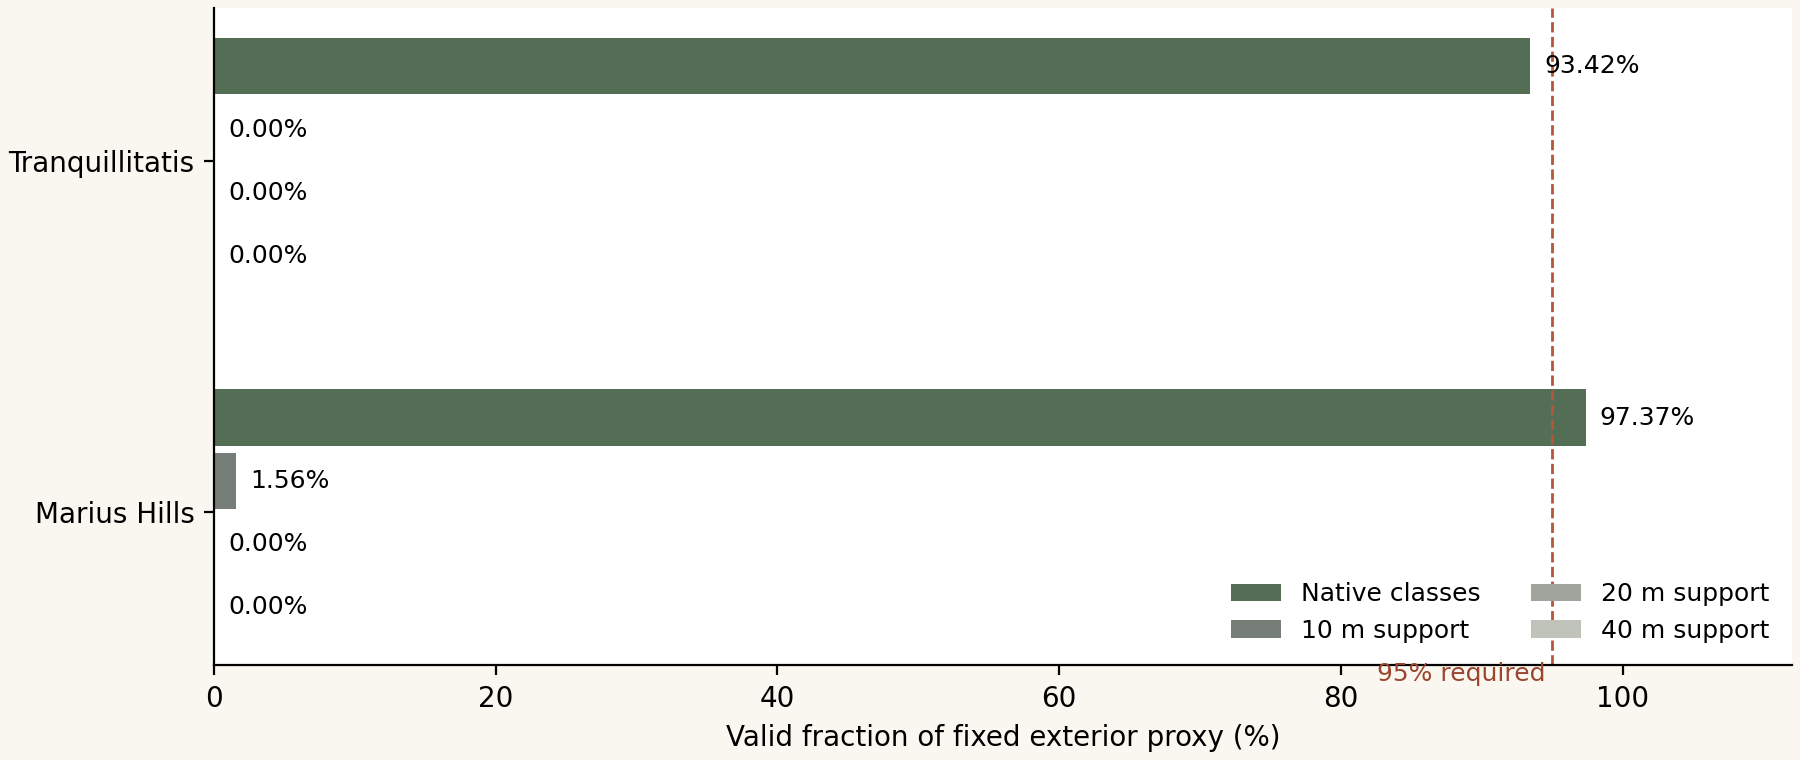
\includegraphics[width=.94\linewidth]{pit-support-summary.png}
\caption{Native quality coverage and usable exterior coverage after neighborhood masking. Values refer to the maximum-funnel circular proxies at the published centers. Posting is 2 m for Tranquillitatis and 4 m for Marius Hills. The dashed line is the declared 95\% requirement.}
\end{figure}

Six complete analytical planes, one per site and support, recover the expected slope within $8.2\times10^{-12}$ degrees and plane-residual standard deviation below $1.3\times10^{-11}$ m. These are numerical controls, not geological reference surfaces. Applying each acquired quality mask rejects the same plane.

The calibration sensitivity matrix contains two funnel diameters per site, five center positions, three supports and two treatments of edited data: 60 runs per site. Offsets of 5 m in either cardinal direction are declared sensitivity distances, not a measured registration-error distribution. No run meets the coverage requirement; the maximum surviving fraction is 1.65\%. These variants were specified after the initial source failures for calibration diagnosis, rather than as a confirmatory experiment.

The current pilot stops here. A later study must qualify exact rims and sources, freeze candidates and independent controls, lock joint and separate nominations from coarse evidence, and evaluate all three pairwise relations on withheld outcomes. That design remains unexecuted. It cannot be filled with synthetic observations or successful software tests.

\clearpage
\section{Replication, transfer and remaining evidence}
\label{app:claims}
A software replication re-executes seven published terrain-ranking sensitivity calculations from Terrestrial Analog Finder's processed feature records \cite{terrainfinder}. The pinned source revision and input hashes are retained with the replication receipt. Across twelve targets and a 469-record Earth reference pool, all seven results agree exactly with the published values. Six calculations drop individual terrain features; the seventh perturbs weights with twenty seeded draws. This reproduces the ranking calculations, not raw DEM acquisition, feature extraction, the source-dependent window experiments or geological relevance. Sixteen upstream similarity tests and nine Analog Atlas scoring tests also pass locally. Software tests do not establish scientific novelty.

An independent adaptation then applies four scalar observables to MIMESIS's existing 3,693 Earth windows: relief, median slope, upper-decile slope and residual roughness. Relief and roughness use $\log_{10}(x+1)$; slopes remain in degrees. Equal-weight RMS distance uses fixed interquartile scales from the 500 m reference pool, with standard deviation as the declared fallback. Incomplete feature vectors are excluded. The adaptation differs from the upstream six-feature definition and is reported separately.

\begin{figure}[h]
\centering
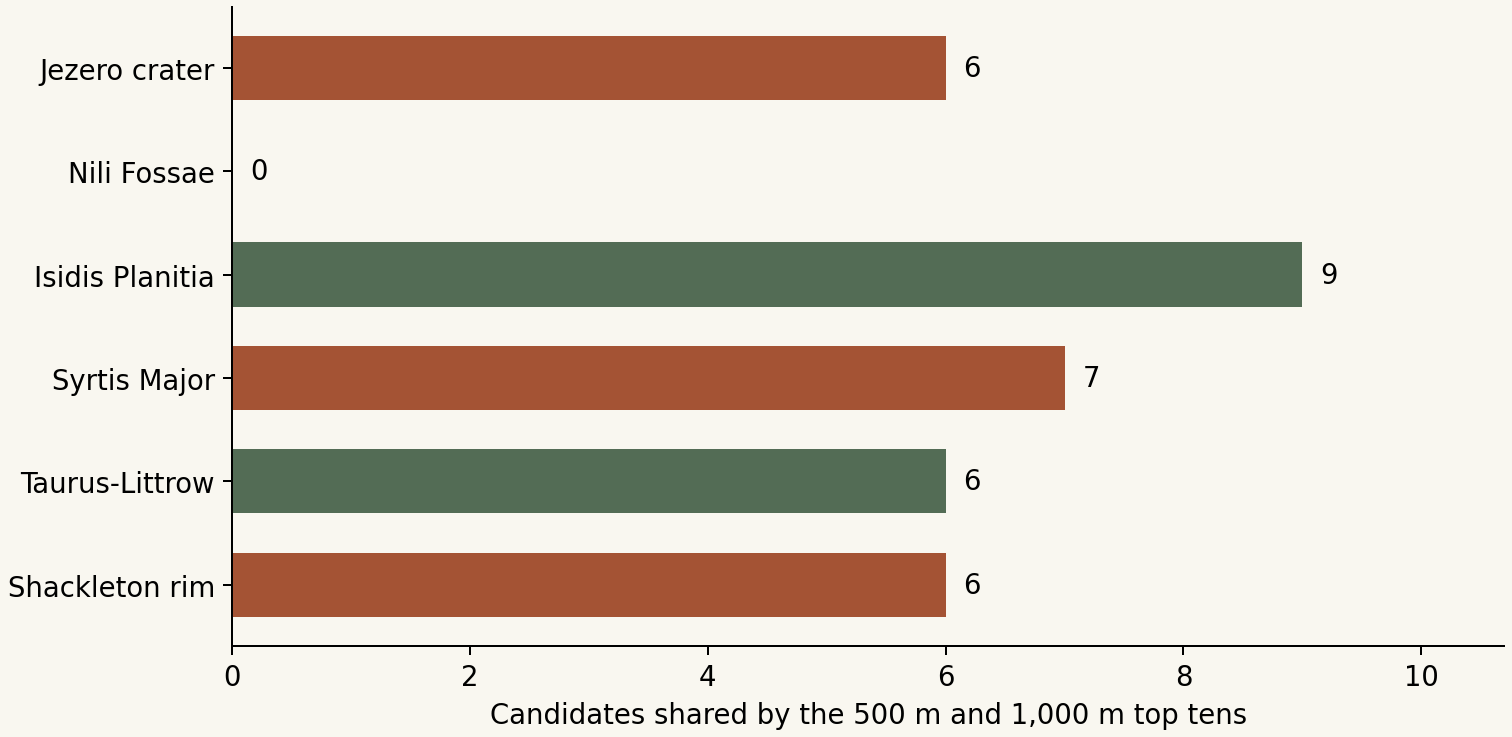
\includegraphics[width=.90\linewidth]{baseline-support-v11.png}
\caption{Exploratory adaptation to MIMESIS records. Shared top-ten Earth windows between 500 m and 1,000 m derivative support. Rust indicates a changed first-ranked window. Four of six targets change their leading candidate; Nili Fossae shares no top-ten candidate across supports. These are previously inspected regional measurements, not feature-scale withheld validation.}
\end{figure}

The result measures ranking sensitivity under this particular scalar baseline. It does not identify an independently validated new analogue or explain a geological cause. Derivative support, native source sampling, missing observations and correlated candidate windows remain limits; a nominal common grid cannot establish common information content.

Source work for a revised pit procedure inventories 278 lunar atlas entries and joins 1,062 Martian catalogue features to 1,377 DTM footprints, excluding one invalid polygon. Nine feature points intersect seven Martian products. Native coverage is audited for five lunar features and nine Martian intersections. Eight US 3DEP entrance-locator crops and a 5 m IGN Lanzarote crop are acquired, but exact rims, local source quality and independent controls are incomplete. IRIDIUMPIT1 and FECNDITATS2 contain native confidence codes outside their published lookups; their coverage is unassessable, not zero. INGENIIPIT conforms to its lookup but fails the original Gaussian support test.

A revised local-plane estimator uses observed centers, at least 80\% of available geometric neighbor weight and condition number at most twenty. The original 95\% scored-sector requirement remains. Its analytical controls and a North Procellarum 2 mask at 40 m are promising numerical checks, not geological calibration. No confirmatory bank, nomination, withheld result or discovery is established. The geographic follow-up adds new calculations to the regional records without completing the feature-scale study.

The four-page application exposes records and exports. Codex assisted Arjun Vijay Prakash with implementation, analysis and writing; independent expert review is not claimed. Original CAVES products retain research-use restrictions and remain outside the public repository and paper archive. A completed software workflow and a completed scientific experiment are separate outcomes.

\end{document}
